\hypertarget{experimental-setup-and-maintenance}{%
\section{Experimental Setup and
Maintenance}\label{experimental-setup-and-maintenance}}

\hypertarget{furnace}{%
\subsection{Furnace}\label{furnace}}

\hypertarget{overview}{%
\subsubsection{Overview}\label{overview}}

The furnace, shown in Figure reffig:furnace\_pic, is an encased stack of
ceramic insulation with cavities cut out to allow space for the heating
elements and the test flask (see Figure reffig:in\_furnace for an
internal diagram of the furnace). The furnace is controlled with
measurements taken at the insulated furnace wall. This design causes the
furnace to have large temperature gradients while in operation. As a
result, the set point temperature and the flask temperature will almost
always differ significantly (as much as 25 K in some cases). Therefore,
set points must be chosen between approximately 10 1. 20 K above the
desired temperature to reach that temperature inside the flask.
\textbf{The reported AIT must be taken from the internal flask
temperature (Thermocouple 4) and NOT the control thermocouple inside the
furnace.} When powered on initially, the furnace may take up to 2 hours
or more to reach a desired temperature and thermally equilibrate. Any
time a desired temperature is reached, allow enough time for thorough
thermal equilibration in the flask; allow extra time during initial
start up.

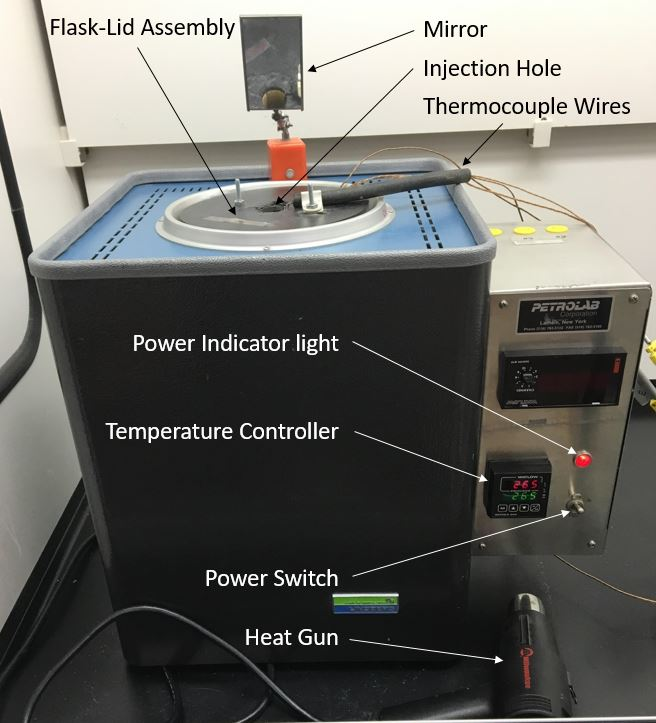
\includegraphics[width=0.5\textwidth]{./Furnace_pic_diagram.jpg}

\hypertarget{furnace-operation}{%
\subsubsection{Furnace Operation}\label{furnace-operation}}

See Figure reffig:furnace\_pic for reference on how to operate the
furnace

\begin{enumerate}
\def\labelenumi{\arabic{enumi}.}
\item
  Power on the furnace with the power switch and use the temperature
  controller to choose a set point temperature
\item
  To change the set point, press the up or down arrows until the desired
  temperature is reached

  \begin{enumerate}
  \def\labelenumii{\arabic{enumii}.}
  \tightlist
  \item
    The lower (green) display is the set point and the upper (red)
    display is the control thermocouple temperature
  \end{enumerate}
\item
  When shutting down, turn off the power switch
\end{enumerate}

\hypertarget{camera}{%
\subsection{Camera}\label{camera}}

\hypertarget{overview-1}{%
\subsubsection{Overview}\label{overview-1}}

Prior to using the experimental setup, all researchers must become
familiar with basic use and operation of the GoPro©~HERO4 Session™
camera and Camera Suite©~software.

GoPro Login:

\begin{itemize}
\tightlist
\item
  \textbf{username/email:} dipprlab.ait@gmail.com
\item
  \textbf{password:} hotflame16
\end{itemize}

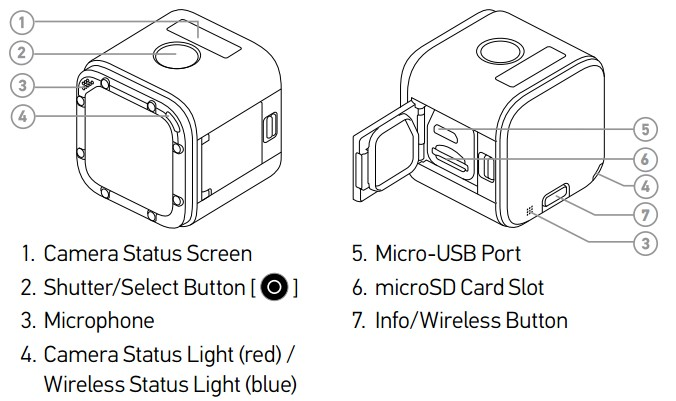
\includegraphics[width=0.5\textwidth]{./Camera_diagram.jpg}

\hypertarget{connecting-to-the-camera}{%
\subsubsection{Connecting to the
camera}\label{connecting-to-the-camera}}

\begin{enumerate}
\def\labelenumi{\arabic{enumi}.}
\tightlist
\item
  Firmly press and release the ``info/wireless'' button on the back of
  the camera (not the red circle) multiple times until you see
  \texttt{APP} or \texttt{APP\ \&\ RC} on the camera status screen
\item
  Press the ``shutter/select'' button (the button with the red circle)
  to confirm your selection
\item
  The ``wireless status'' (blue) light will begin flashing. This
  indicates the camera is broadcasting a Wi-Fi signal
\item
  When first powering on the camera, ensure it is sufficiently charged.
  If not, immediately plug it in to charge it.
\item
  In the lower-right-hand corner of the desktop you will see an icon for
  internet connections. The computer should automatically connect to the
  Wi-Fi but if it does not, connect to the Wi-Fi using the following
  credentials:

  \begin{itemize}
  \tightlist
  \item
    Network Name: \texttt{ait\_cam\_2020}
  \item
    Password: \texttt{hotflame16}
  \end{itemize}
\item
  Open the Camera Suite©~app (There should be a shortcut on the
  desktop.)
\item
  If the app does not immediately try to connect to the camera, go to
  the pop up dialogue box and select \texttt{Hero\ 4} from the drop-down
  menu and click on \texttt{connect\ to\ camera}.

  \begin{itemize}
  \tightlist
  \item
    The app should attempt to connect to the camera.
  \end{itemize}
\item
  Press the ``info/wireless'' button to make the camera accept the
  connection from the computer.
\item
  On the right side of the Camera Suite© app, the camera info along with
  control buttons should appear. This means the camera is connected.
\end{enumerate}

\hypertarget{camera-operation}{%
\subsubsection{Camera Operation}\label{camera-operation}}

All operations may be done remotely via Wi-Fi or directly with the
``info/wireless'' and ``shutter/select'' buttons on the camera. For
experimental purposes, only basic operations will be covered. For more
detail on camera operation please see the GoPro© HERO4 Session™ camera
operation manual in the \texttt{docs} section of the \texttt{ait\_exp}
repository.

\begin{enumerate}
\def\labelenumi{\arabic{enumi}.}
\tightlist
\item
  The ``shutter/select'' button toggles recording or standby; the camera
  will automatically shut off after a few seconds on standby
\item
  If the camera is remotely controlled, the on screen red button toggles
  recording or standby
\item
  During recording, the camera will not allow viewing via preview mode.
  This is due to the high frame rate of our experiments
\item
  Captured video may be reviewed, downloaded and managed remotely with
  camera browser button on the top left corner of the screen (make sure
  you hit ``refresh'' to update the contents in the camera).
\item
  The camera may be powered on and off remotely with the power button on
  the top right corner of the screen. The camera should be powered off
  between experiments or when not in use
\end{enumerate}

\hypertarget{shutdown}{%
\subsubsection{Shutdown}\label{shutdown}}

\begin{enumerate}
\def\labelenumi{\arabic{enumi}.}
\item
  Press the ``info/wireless'' button until the camera status screen
  reads ``Turn Wi-Fi Off''
\item
  Press the ``shutter/select'' button to confirm your selection

  \begin{itemize}
  \tightlist
  \item
    The ``wireless status'' (blue) light will stop flashing
  \end{itemize}
\item
  Press the ``info/wireless'' button until the camera status screen
  reads ``Exit''
\item
  Press the ``shutter/select'' button to confirm your selection
\item
  The camera will shutdown
\end{enumerate}

\hypertarget{camera-placement-and-removal}{%
\subsubsection{Camera Placement and
Removal}\label{camera-placement-and-removal}}

To mount the camera on the furnace:

\begin{enumerate}
\def\labelenumi{\arabic{enumi}.}
\tightlist
\item
  Lift the tab on the corner of the camera cage
\item
  Insert the camera from the front of the cage with the
  ``shutter/select'' button facing up.
\item
  Snap the tab back to lock the camera into place.
\end{enumerate}

To remove the camera from the furnace:

\begin{enumerate}
\def\labelenumi{\arabic{enumi}.}
\tightlist
\item
  Lift the tab on the corner of the camera cage
\item
  Slide the camera out of the cage.
\end{enumerate}

\hypertarget{batteries}{%
\subsubsection{Batteries}\label{batteries}}

\begin{enumerate}
\def\labelenumi{\arabic{enumi}.}
\tightlist
\item
  USB chargers and cables are available for the camera
\item
  Charge batteries as needed. A charge above 80\% is required before
  running an experiment to ensure the battery doesn't die during an
  experiment.
\item
  Do not overcharge the camera battery. Do not leave any battery
  charging overnight.
\end{enumerate}

\hypertarget{pressure-vessel}{%
\subsection{Pressure Vessel}\label{pressure-vessel}}

\hypertarget{changing-the-rupture-disk}{%
\subsubsection{Changing the rupture
disk}\label{changing-the-rupture-disk}}

We use 1100 alloy extra thin aluminum foil as a rupture disk. This
material has been shown to be effective in preventing catastrophic
failure in the vessel. This section outlines how to change and test the
rupture disk. (See Figures reffig:rupture disk\_assemble and
reffig:rupture\_disk for reference)

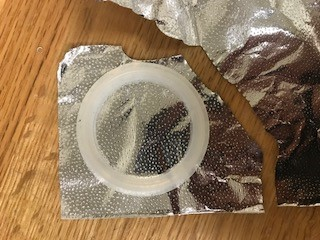
\includegraphics[width=0.5\textwidth]{./o_ring_on_foil.jpg}

\begin{enumerate}
\def\labelenumi{\arabic{enumi}.}
\item
  Remove the O-ring and the TC outlet ring from the pressure vessel by
  removing the TC clamp (See Figure reffig:rupture\_disk)
\item
  place the O-ring on a piece of extra thin 1100 alloy aluminum foil

  \begin{itemize}
  \tightlist
  \item
    \textbf{Do NOT use the aluminum foil used for wrapping the flask, it
    is far too strong and may lead to a catastrophic failure of the
    vessel}
  \end{itemize}
\item
  Rip the foil around the O-ring so it roughly matches the area of the
  O-ring
\item
  Sandwich the ripped foil in between the O-ring and the outlet ring
\item
  Place the combined rings and foil on the rupture outlet on the
  pressure vessel and fold any excess foil over the rupture outlet on
  the pressure vessel
\item
  Secure the assembly on the pressure vessel using the TC clamp
\item
  The foil should appear smooth across the rupture surface without any
  folds or crumpled spots
\item
  The studded surface may still be apparent; this is normal
\end{enumerate}

\hypertarget{rotameter}{%
\subsection{Rotameter}\label{rotameter}}

\hypertarget{disassembling-the-rotameter}{%
\subsubsection{Disassembling the
Rotameter}\label{disassembling-the-rotameter}}

\begin{enumerate}
\def\labelenumi{\arabic{enumi}.}
\tightlist
\item
  gently squeeze plastic cover and pull off
\item
  using a small Allen wrench (\textasciitilde{} 0.060") loosen the set
  screw on the rotameter dial and remove it
\item
  remove ring around the valve
\item
  use a 7/16" wrench to remove the valve assembly at the bottom of the
  rotameter
\item
  use 2 3/8" wrench and a 7/16" wrench to remove the inner part of the
  valve assembly
\item
  Unscrew the needle valve by hand so the valve assembly is completely
  disassembled (there should be 3 parts)
\item
  (DO NOT REMOVE THE O-RINGS)
\item
  use a 5/8" wrench to remove the brass hose fitting at the inlet to the
  rotameter
\item
  use a small screwdriver to pry off the plastic cap at the top of the
  rotameter
\item
  use a 1/8" Allen wrench to loosen the top screw over the rotameter
  sight glass to allow the sight glass to be removed
\item
  carefully remove the sight glass by tipping the top away from the
  rotameter and pulling up out of the bottom portion
\end{enumerate}

\hypertarget{flask-and-lid}{%
\subsection{Flask and Lid}\label{flask-and-lid}}

\begin{enumerate}
\def\labelenumi{\arabic{enumi}.}
\item
  textbfLatex or nitrile gloves and safety glasses are required while
  working with the flask/lid assembly
\item
  Using the TADA\_UI, check the temperature of the furnace to ensure
  safe handling before changing the flask
\item
  The temperature should be close to ambient lab temperature
\item
  Do not perform maintenance or change the flask unless the internal
  temperature of the furnace is below \(40^circ C\)
\item
  The flask in the furnace must be exchanged for a clean flask in the
  following situations:
\item
  The next experiment will be for a different compound
\item
  The next experiment will be for a new container of the same compound
\item
  There is reason to suspect that the flask has become contaminated or
  substantially dirty
\item
  The flask has been used for 10 runs without being cleaned
\item
  Once the AIT has been found for a compound, the final measurements
  should be repeated with a clean flask to verify the results
\item
  Disassembling the Flask and Lid
\item
  textbfThe furnace may be too hot to open for several hours after an
  experiment
\item
  Unplug the thermocouples from the furnace
\item
  Once the furnace is cool, remove flask/lid assembly
\item
  Loosen (do NOT remove) the nut that secures the bracket and the rubber
  hose to the top of the furnace with a wrench
\item
  Move the bracket out of the way and remove Thermocouple 4 (along with
  the rubber hose) from the top of the furnace
\item
  Move the mirror out of the way to allow the flask/lid assembly to come
  out. Likewise ensure that the ARIA is out of the way
\item
  Grip the assembly with both hands by the screws on top and pull
  directly upward
\item
  textbfNOTE: The flask/lid assembly is heavy and pulling it\\
  out can be awkward. Please ask someone to help you remove it if you
  are at all unsure about removing the assembly
\item
  The flask/lid assembly should easily come out of the furnace without
  catching on anything
\item
  textbfCarefully set the assembly on a table or other stable surface
  with the flask on top (See Figure reffig:f\_lid\_done)
\item
  Ensure the bracket screw is loose
\item
  Remove the circular spring from its groove and slide the ceramic
  halves of the lid apart sufficiently to allow the flask to be removed
\item
  Remove flask from lid assembly and remove all of the aluminum foil and
  thermocouples from the flask
\item
  Discard the used aluminum foil in a normal trash can and set aside the
  thermocouples in the hood or on a surface where they will not catch on
  anything or become damaged
\item
  textbfAlways store bulb flasks on the drying rack above the sink or
  appropriately secured to a ring stand (see ``Flask Cleaning'' section)
\item
  textbfNOTICE: Every time the flask and lid are disassembled, check the
  thermocouples and thermocouple wiring for damage or fraying that may
  affect thermocouple performance. If needed, replace the thermocouples
  before assembling the flask and lid.
\item
  Assembling the Flask and Lid
\item
  Use the figures in this section as a reference when putting together
  the assembly
\item
  Use a textbfclean, 500 ml, round bottom, long neck, bulb flask
  (PYREXtextsuperscripttextcopyright 500mL Long Neck Boiling Flask,
  Round Bottom, Tooled Mouth, Product No.: 42801.500 from Corning Inc.)
\item
  If dirty, wash out the flask using soap and water and dry as much as
  possible (see ``Flask Cleaning'' section); be sure to rinse thoroughly
\item
  Any leftover water will boil away when the furnace heats up and before
  any measurements are taken
\item
  Wrap entire flask in aluminum foil with thermocouples at the bottom,
  side and top of the round part of the flask (thermocouples should be
  touching the glass directly) (Refer to Figure reffig:wrap)
\item
  NOTE: The more reflective side of the foil should always be facing
  inward
\item
  Start by getting a long strip of aluminum foil (12" long or so)
\item
  Use a utility knife to poke a small hole (just big enough to poke the
  bead through) near the middle of the foil and insert thermocouple 3
  through the foil so the bead sits at the bottom of the flask and then
  wrap the foil around the bottom (1 and 2)
\item
  Slide thermocouple 2 down to the approximate middle/equator of the
  flask between the flask and foil and run a couple of inches around the
  equator so that it stays in place\\
\item
  Use a second piece of foil to wrap further up the flask, ensuring the
  thermocouple wires run parallel up the side of the flask (3)
\item
  Place thermocouple 1 at the top of the bulb of the flask (textbfNOT on
  the neck of the flask) and use a third piece of foil to wrap around
  the top starting at the middle (4)
\item
  Add an additional layer of foil around the flask so the wires are
  covered and run parallel when wrapping is finished

  \begin{enumerate}
  \def\labelenumii{(\arabic{enumii})}
  \setcounter{enumii}{4}
  \tightlist
  \item
  \end{enumerate}
\item
  Wrap additional foil around the neck of the flask to cover it
  completely and secure flask in lid assembly
\item
  The thermocouple wires should emerge from the foil covering near the
  top (but not at the top) of the flask neck, allowing them to run
  between the two ceramic halves of the lid assembly (6)
\end{enumerate}

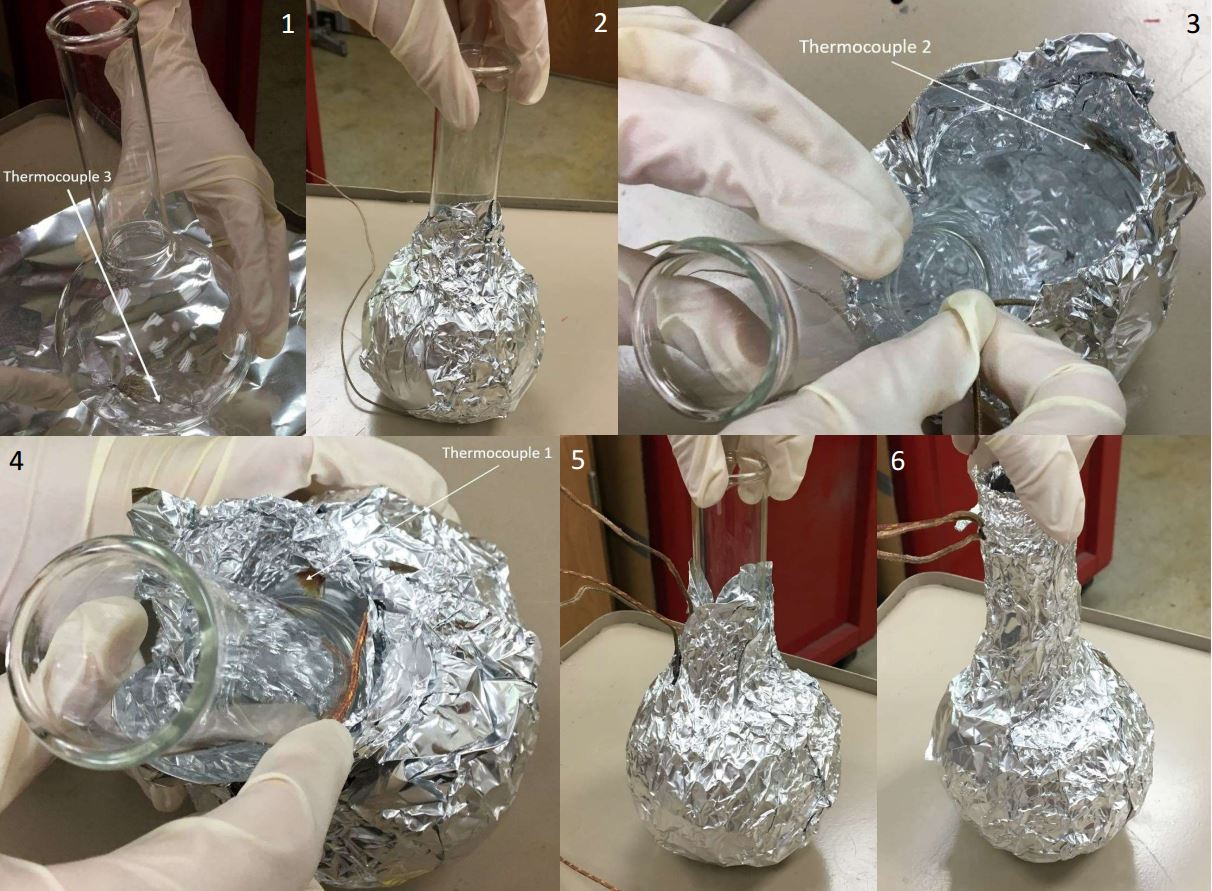
\includegraphics[width=0.5\textwidth]{./wrap.jpg} Steps for wrapping the flask in foil
